\chapter{Estudo de Caso}
O estudo de caso que será usado para validar os métodos de Aprendizagem de Máquina com Aprendizagem Incremental é baseado em um problema real do Ministério da Agricultura, Pecuária e Abastecimento (MAPA). Este ministério é responsável  "pela gestão das políticas públicas de estímulo à agropecuária, pelo fomento do agronegócio e pela regulação e normatização de serviços vinculados ao setor" \cite{mapa}. Um dos objetivos do MAPA é garantir a segurança alimentar do povo brasileiro além de suportar a produção de exportação, garantindo o sucesso dos produtos brasileiros no mercado internacional.

Uma das atribuições do Ministério da Agricultura é velar pela segurança dos produtos agropecuários que entram e saem do país. Para isto existe o Sistema de Vigilância Agropecuária Internacional (Vigiagro) que é vinculado a Secretaria de Defesa Agropecuária. O vigiagro "atua na inspeção e fiscalização do trânsito internacional de vegetais, seus produtos e subprodutos. A fiscalização é feita nos portos, aeroportos internacionais, postos de fronteira e aduanas especiais" \cite{vigiagro}.

Neste contexto o vigiagro tem a atribuição fiscalizar todas as importações e exportações de produtos agropecuários do Brasil. Cada importação/exportação gera um requerimento, um documento onde o exportador/importador informa que realizará uma transação comercial internacional de um produto que está sobre vigilância do Vigiagro. Todos os requerimentos são inseridos no Sistema de Informações Gerenciais (SIGVIG). Os funcionários do Ministério então verificam vários itens, alguns de cunho documental e outros de cunho físico do produto comercializado. Caso haja alguma inconformidade o fiscal que avalia o requerimento gera um Termo de Ocorrência (TO) explicando a natureza e razão do erro encontrado, seja documental ou físico. Caso não haja nenhum erro o TO gerado consta que não houve erro em nenhum dos critérios avaliados.

O problema de todo este processo é que no Brasil a quantidade de requerimentos gerada é enorme. O processo de fiscalização é extremamente trabalhoso e demanda muito tempo dos fiscais. Propõe-se utilizar métodos de Aprendizado de Máquina para criar um sistema que auxilie na fiscalização, diminuindo o tempo de processamento dos requerimentos e aumentando a qualidade da fiscalização. Este sistema deve ser capaz de analisar todos os requerimentos feitos associados com o resultado da fiscalização, deferimento ou indeferimento do processo. Através desta análise deve ser possível classificar os exportadores/importadores em três categorias: Alta Conformidade, Média Conformidade e Baixa Conformidade. Através destes três rótulos é possível criar políticas de fiscalização que foquem os esforços nos comerciantes que geralmente possuem baixa conformidade em seus requerimentos, fazendo com que os comerciantes que sempre possuem conformidade tenham seus processos agilizados e os que possuem baixa conformidade tenham seus requerimentos avaliados cuidadosamente. 

Os dados que são relevantes para a construção deste sistema classificador é proveniente da união de dois relatórios gerados pelo SIGVIG: O relatório de todos Requerimentos de um determinado período de tempo com todos os Termos de Ocorrência correspondentes a estes requerimentos. A combinação destes dois relatórios fornece as características do importador/exportador, as características do produto negociado e o resultado da avaliação deste requerimento pelos fiscais do MAPA.

A figura 12 é um exemplo de como será o conjunto de dados que deve ser avaliado pelo sistema classificador. Ela consiste em 37 registros que são a combinação das informações entre Requerimentos e Termos de Ocorrência de produtos de importação.

\begin{figure}[!h]
\centering
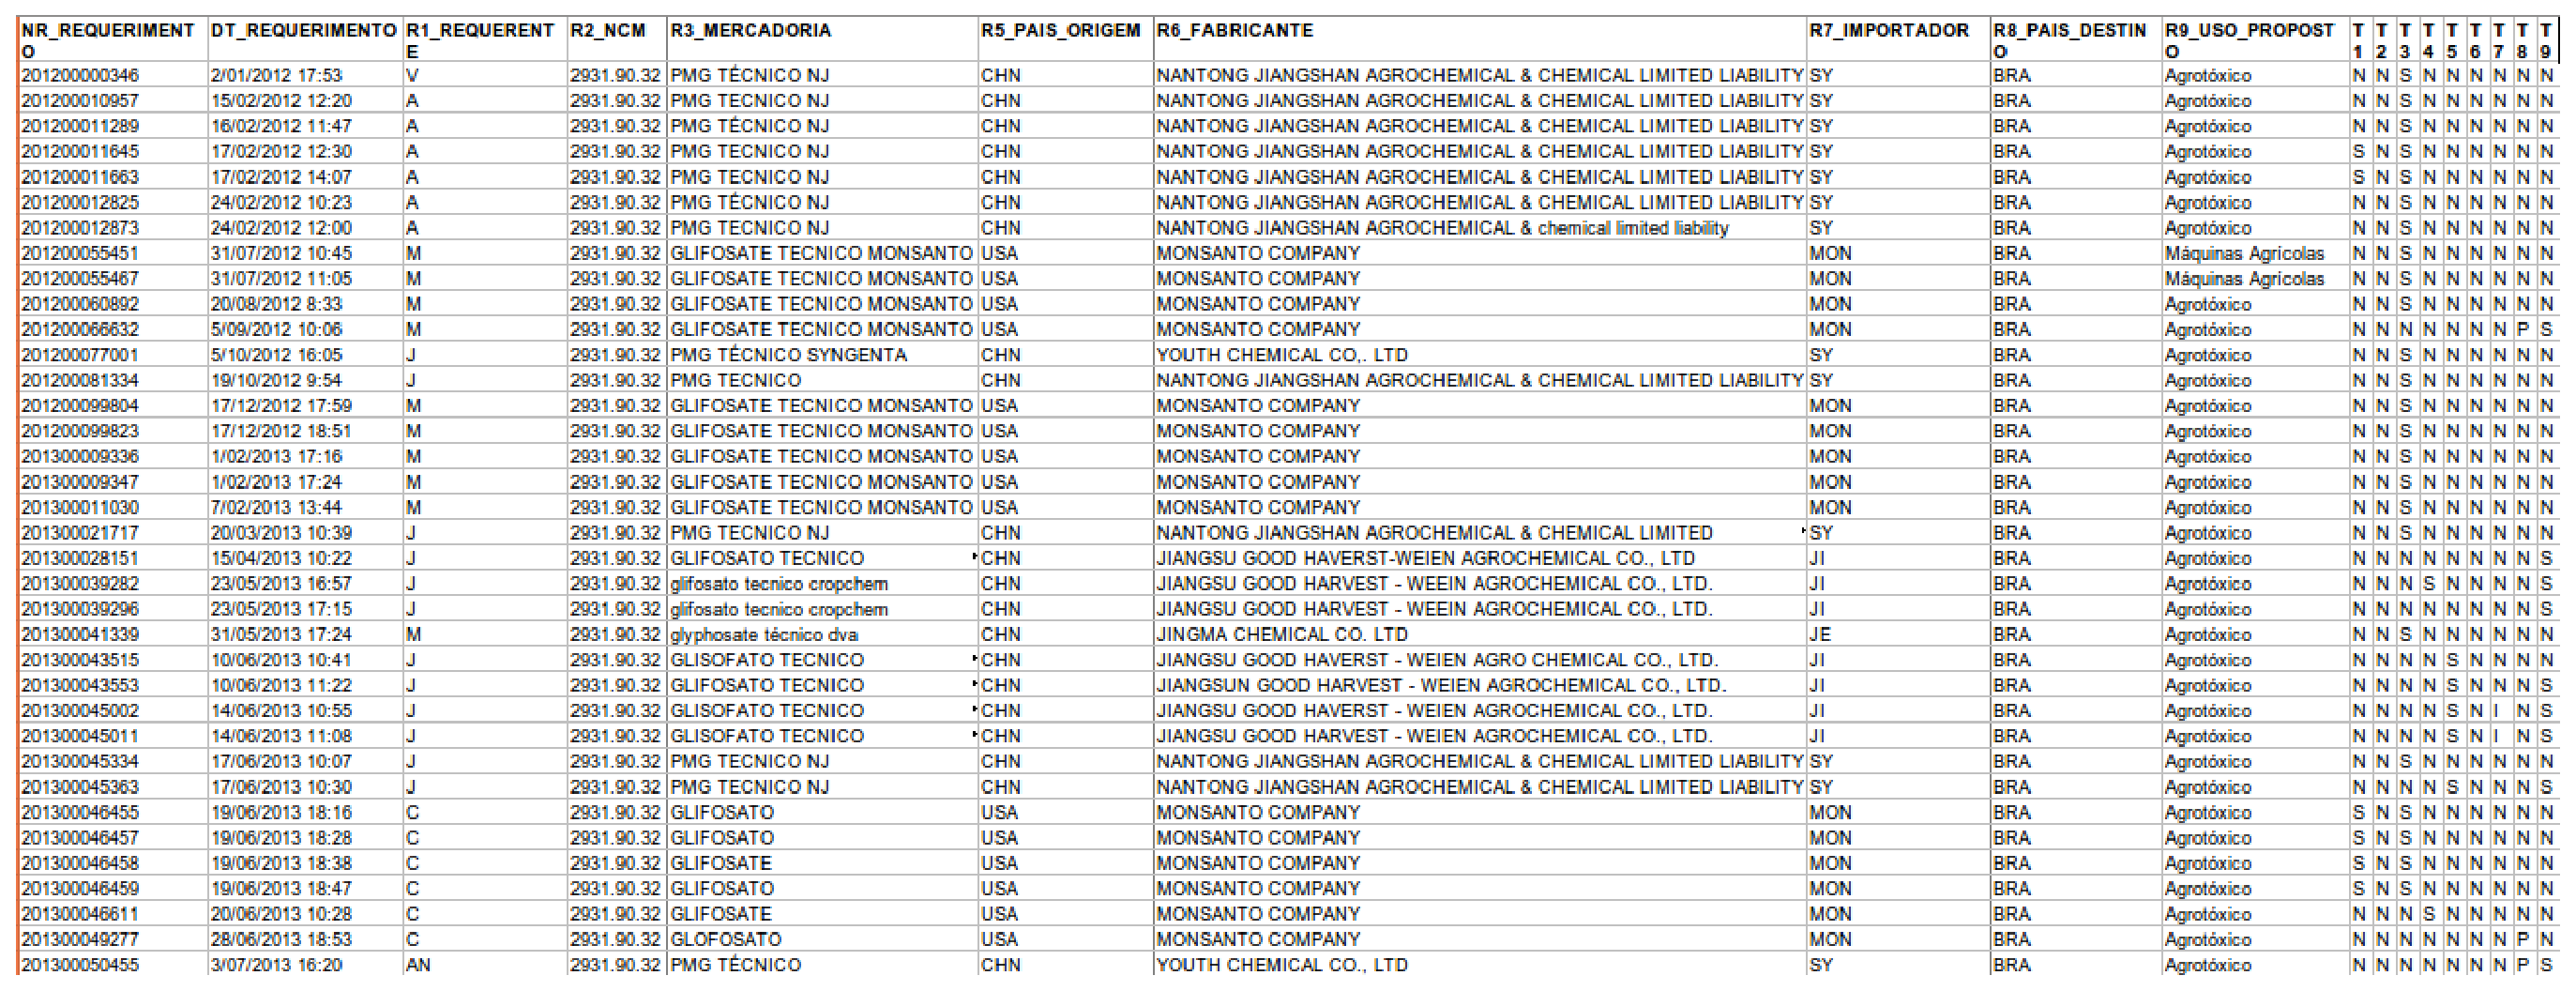
\includegraphics[keepaspectratio=true,scale=0.40]
{figuras/tabelaMapa.eps}
\caption{Dados de Exemplo}
\label{tabelaMapa}
\end{figure}

\begin{enumerate}
\item NR REQUERIMENTO: É um atómo numérico que identifica unicamente o requerimento. Os quatro primeiro dígitos são relativos ao ano em que o requerimento foi feito.
\item DT REQUERIMENTO: É uma sequência unidimensional de categóricos, um campo texto. Nesta coluna consta o momento no tempo em que este requerimento foi feito.
\item  R1 REQUERENTE: Sequência textual que identifica unicamente o empresário requerente.
\item  R2 NCM: NCM siginifica Nomenclatura Comum do Mercosul. Este código identifica o produto ou categorias de produtos para fins de padronizar operações comerciais no mercosul. É uma sequência unidimensional de categóricos.
\item R3 MERCADORIA: Nome do produto comercializado. É uma sequência unidimensional de categóricos.
\item  R5 PAIS ORIGEM: Sigla que corresponde ao país de origem do produto importado. É um átomo categórico.
\item R6 FABRICANTE: Corresponde ao nome da empresa fabricante do produto importado. É uma sequência unidimensional de categóricos.
\item R7 IMPORTADOR: Corresponde ao importador do produto no país de origem. É uma sequência unidimensional de categóricos.
\item R9 USO PROPOSTO: Átomo categórico que corresponde ao objetivo de utilização do produto importado.
\item T0: Átomo categórico que corresponde ao objetivo de utilização do produto importado.
\end{enumerate}



































